\providecommand{\relativeRoot}{../..}
\documentclass[\relativeRoot/main.tex]{subfiles}
\graphicspath{
    {\subfix{./figures/}}
}


\begin{document}

\section{Head and Neck Squamous Cell Carcinoma}
\label{sec:intro:hnscc}

\subsection*{Description}
\label{subsec:intro:hnscc:description}

All body surfaces and cavities are covered in a type of tissue called \emph{epithelium}. For example, both the skin and the lungs are lined with epithelial cells. Of those cells, three different basic types can be distinguished:
\begin{enumerate*}[label={(\arabic*)}]
    \item \textbf{Squamous} (from \emph{squama}, Latin for ``scale'') cells are flat and thin, while 
    \item \textbf{cuboidal} cells are approximately as thick as they are wide and lastly
    \item \textbf{columnar} epithelial cells are column-like and hence much taller than wide
\end{enumerate*}.
They often have a hexagonal shape when viewed from above (meaning perpendicular to the surface they cover) and are close-packed with little to no intercellular space \cite{marieb_human_1995}.

Malignancies -- or more precisely \emph{malign neoplasms} -- that develop in squamous cells of the epithelium are called \gls{scc}. As many parts of the human body are covered with such cells, there exists a respective variety of locations where \gls{scc} can arise. E.g., it is common in the lung, skin or the vagina. But it may also arise in the \emph{mucosa} inside the mouth and upper respiratory tract. In that case, the malignancy is termed \gls{hnscc}.

\gls{hnscc} is the most common type of head and neck cancer, and the sixth most common type of cancer worldwide with an incidence of almost 900,000 new cases in 2018, of which 450,000 resulted in deaths. \cite{johnson_head_2020,ferlay_estimating_2019,bray_global_2018}. Air pollutants, tobacco and alcohol abuse have been linked to an increased risk for \gls{hnscc} \cite{johnson_head_2020,wong_cancers_2014}, as well as an infection with the \gls{hpv}, especially the subtype \gls{hpv}-16 \cite{hennessey_human_2009}.

\subsection*{Spread through the Lymphatic System}
\label{subsec:intro:hnscc:lymph_spread}

\begin{figure}
    \centering
    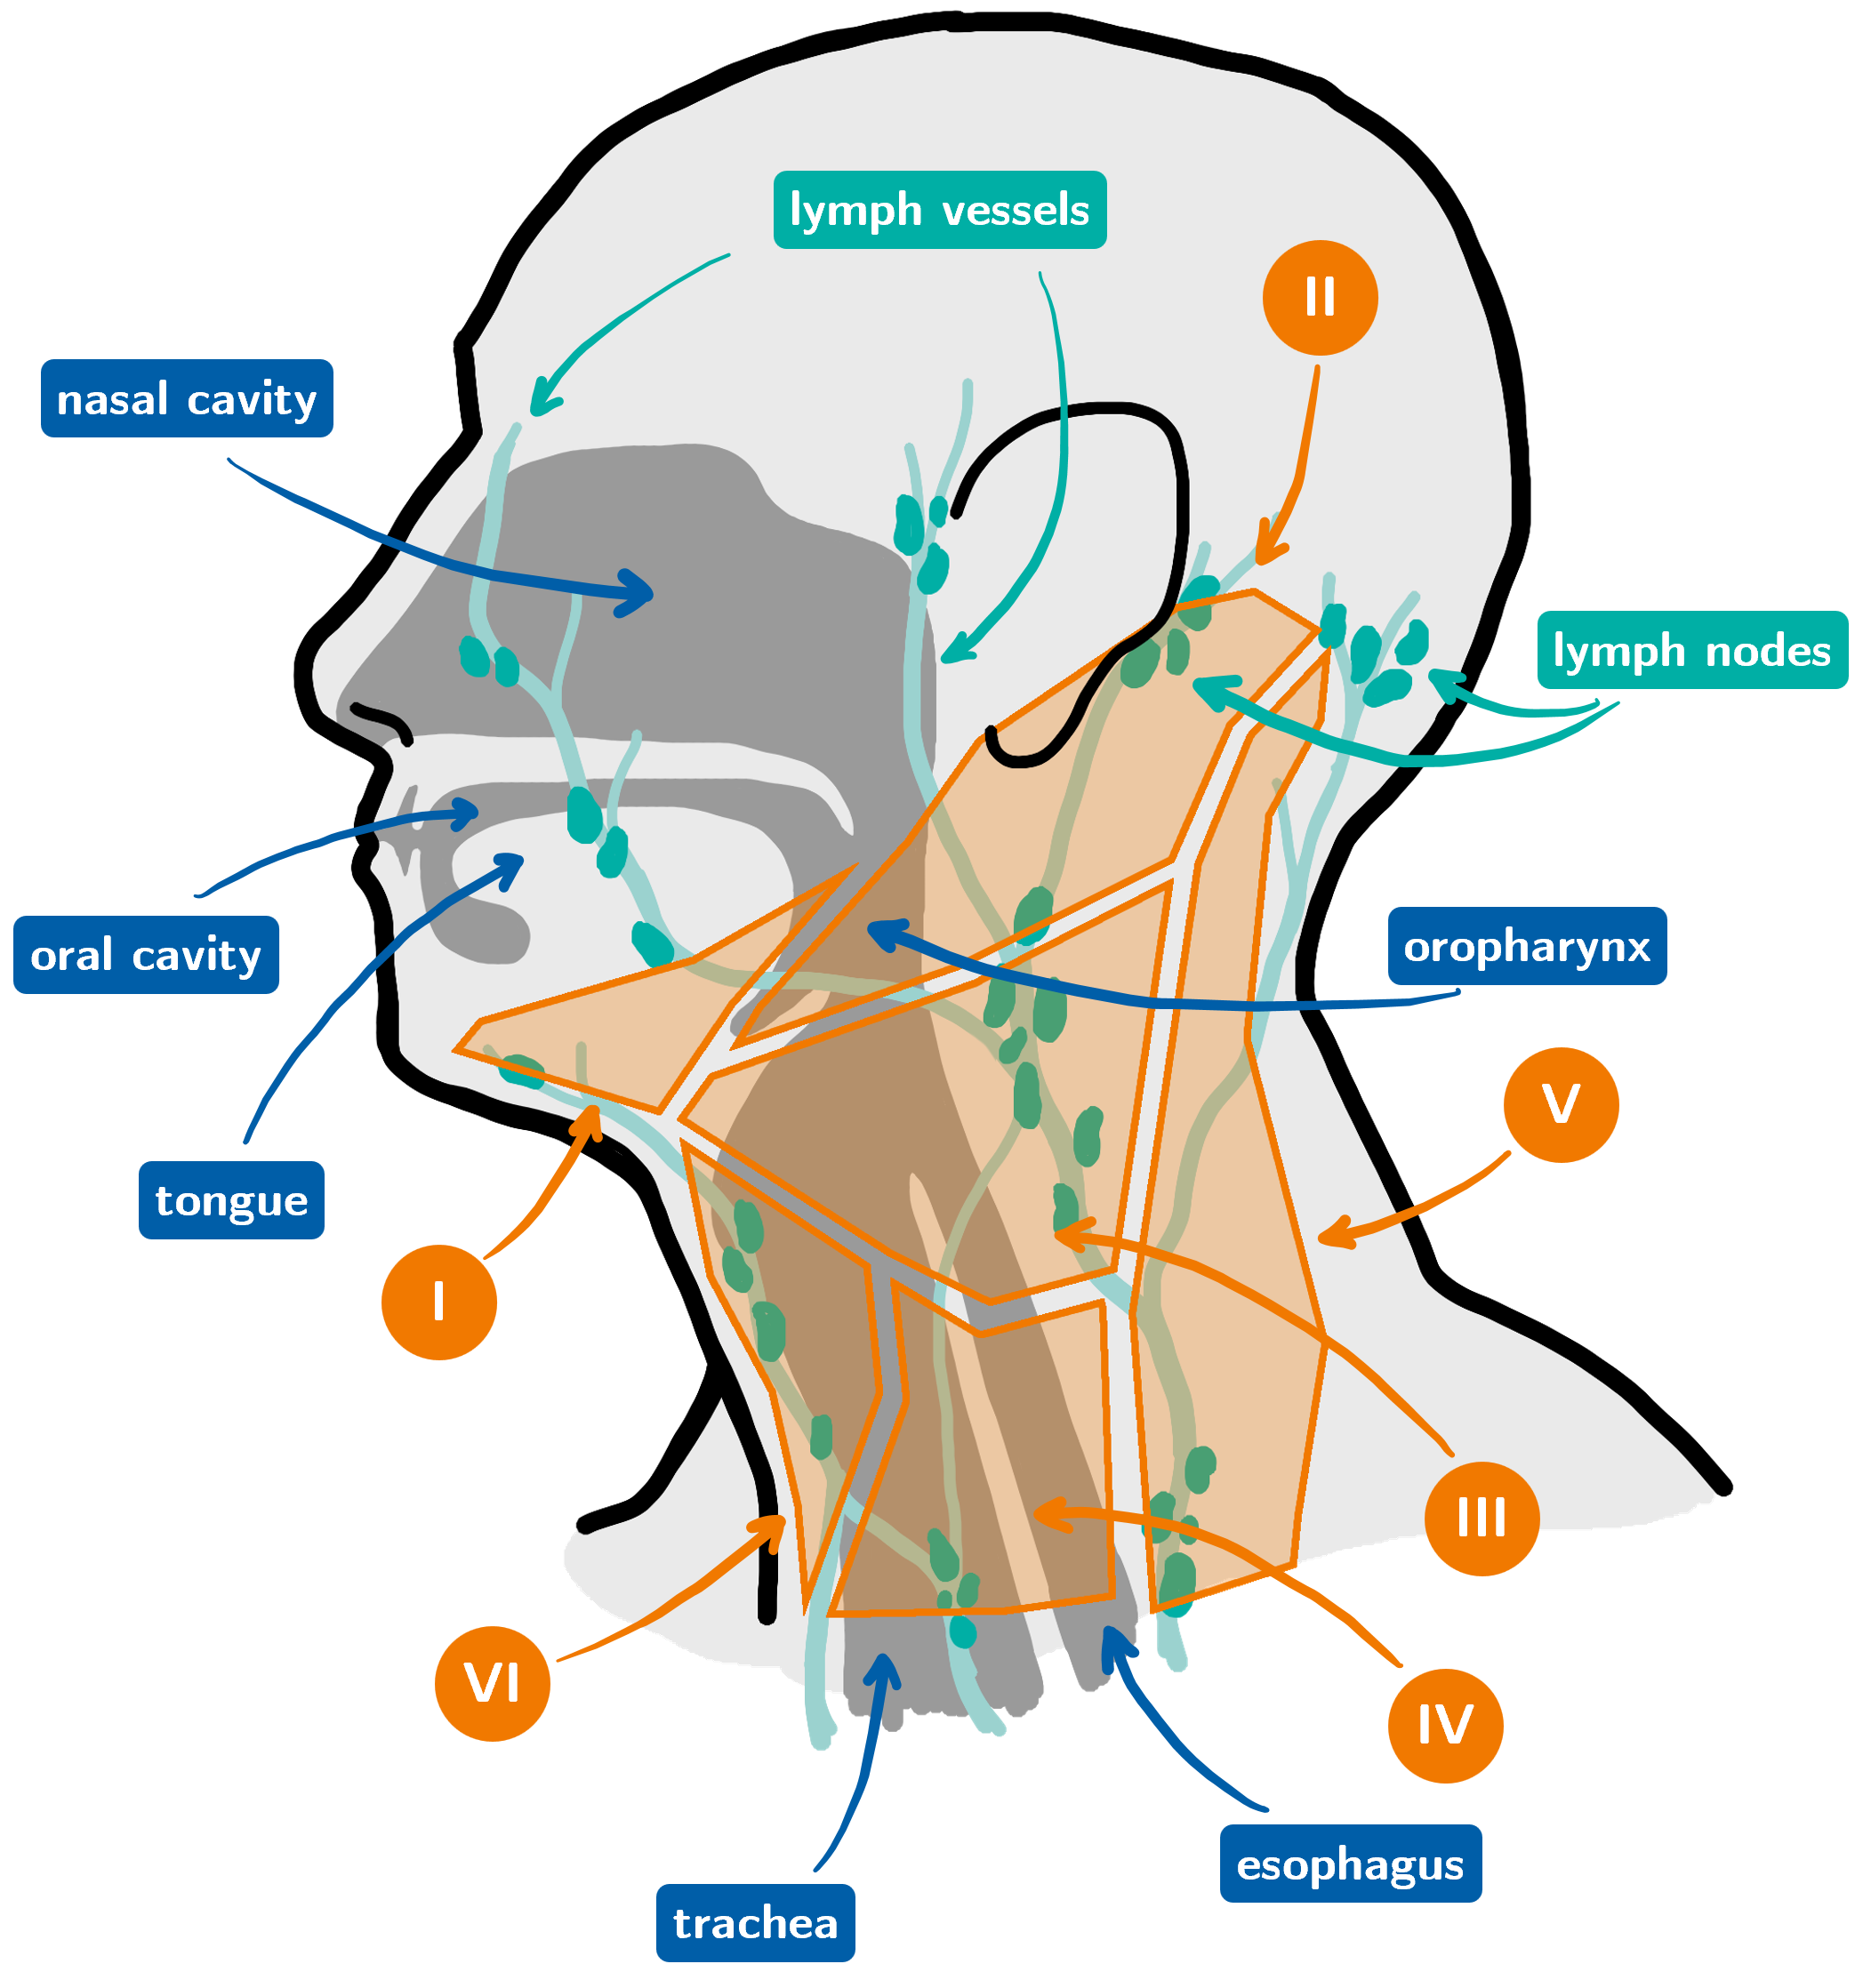
\includegraphics[width=\textwidth]{figures/head_and_neck_labelled.png}
    \caption[
        Schematic drawing of the head and neck region.
    ]{
        Schematic drawing of the lymphatic network in the head and neck region. The shaded area in dark gray depicts a sagittal cross-section of the upper respiratory track and is labelled with blue arrows and tags. Lymphatic vessels are drawn in light green with dark green lymph nodes attached to them. On top, using a transparent shade of orange and orange outlines, we have roughly indicated the location of the \glspl{lnl}. They group the lymph nodes in the head and neck region into regions that are separated by anatomical features not shown in this schematic. E.g., the inferior border of the hyoid bone separates \gls{lnl} II and III axially. The diagram has been roughly traced from the anatomical illustrations in \citeauthorandlink{lengele_anatomical_2007}.
    }
    \label{fig:intro:schematics_head}
\end{figure}

The lymphatic system is a vascular network that is imbued in most human tissue alongside the circulatory system (except e.g. the brain). It consists of thin-walled capillaries that are more preamble than blood vessels. Extracellular fluid, with which cells are provided by circulatory vessels, and into which they release waste products, drains into these permeable lymphatic capillaries and is transported back into the blood \cite{wissmann_pathways_2006,oliver_rediscovery_2002}. Also included in the lymphatic system are organs and structures that play an important role in the human immune response. For example, the lymph nodes, which are located at numerous junctions of afferent lymphatic vessels. Particles from the incoming fluid are filtered out, and it is then drained into the efferent lymphatic vessel \cite{willard-mack_normal_2006}.

Due to this filtering function, lymph nodes also receive cells that an \gls{hnscc} may have shed. In contrast to normal epithelial cells, those of \glspl{scc} exhibit factors that suppress \emph{anoikis}, a form of programmed cell death initiated when these cells become detached from their surroundings \cite{peltanova_effect_2019}. Consequently, live cells detached from the tumor may flow into lymphatic vessels, and get filtered out by the lymph nodes, where they then start to proliferate.

Linked to this briefly outlined process of lymph node metastasis is a significantly lower survival of \gls{hnscc} patients and hence it is considered one of the most prognostic factors \cite{jones_level_1994,lim_distributions_2006,takes_staging_2004}.

\end{document}
